% --------------------------------------------------------------
% This is all preamble stuff that you don't have to worry about.
% Head down to where it says "Start here"
% --------------------------------------------------------------
 
\documentclass[12pt]{article}
 
\usepackage[margin=1in]{geometry} 
\usepackage{amsmath,amsthm,amssymb}
\usepackage[margin=1in]{geometry} 
\usepackage{amsmath,amsthm,amssymb}
\usepackage[T1]{fontenc} %escribe lo del teclado
\usepackage[utf8]{inputenc} %Reconoce algunos símbolos
\usepackage{lmodern} %optimiza algunas fuentes
\usepackage{graphicx}
\graphicspath{ {images/} }
\usepackage{tikz}
\usepackage[]{algorithm2e}
\usepackage{amsmath}
\usepackage{hyperref} % Uso de links
 
\newcommand{\N}{\mathbb{N}}
\newcommand{\Z}{\mathbb{Z}}
 
\newenvironment{theorem}[2][Theorem]{\begin{trivlist}
\item[\hskip \labelsep {\bfseries #1}\hskip \labelsep {\bfseries #2.}]}{\end{trivlist}}
\newenvironment{lemma}[2][Lemma]{\begin{trivlist}
\item[\hskip \labelsep {\bfseries #1}\hskip \labelsep {\bfseries #2.}]}{\end{trivlist}}
\newenvironment{exercise}[2][Exercise]{\begin{trivlist}
\item[\hskip \labelsep {\bfseries #1}\hskip \labelsep {\bfseries #2.}]}{\end{trivlist}}
\newenvironment{problem}[2][Problem]{\begin{trivlist}
\item[\hskip \labelsep {\bfseries #1}\hskip \labelsep {\bfseries #2.}]}{\end{trivlist}}
\newenvironment{question}[2][Question]{\begin{trivlist}
\item[\hskip \labelsep {\bfseries #1}\hskip \labelsep {\bfseries #2.}]}{\end{trivlist}}
\newenvironment{corollary}[2][Corollary]{\begin{trivlist}
\item[\hskip \labelsep {\bfseries #1}\hskip \labelsep {\bfseries #2.}]}{\end{trivlist}}

\newenvironment{solution}{\begin{proof}[Solution]}{\end{proof}}
 
\begin{document}
 
% --------------------------------------------------------------
%                         Start here
% --------------------------------------------------------------
 
\title{Learning Coursework: Task 2 report}



\maketitle
\subsection*{2.3 - Polygon A classification}

\begin{figure}[!htb]
\centering
\tikzset{%
  every neuron/.style={
    circle,
    draw,
    minimum size=1cm
  },
  neuron missing/.style={
    draw=none, 
    scale=4,
    text height=0.333cm,
    execute at begin node=\color{black}$\vdots$
  },
}

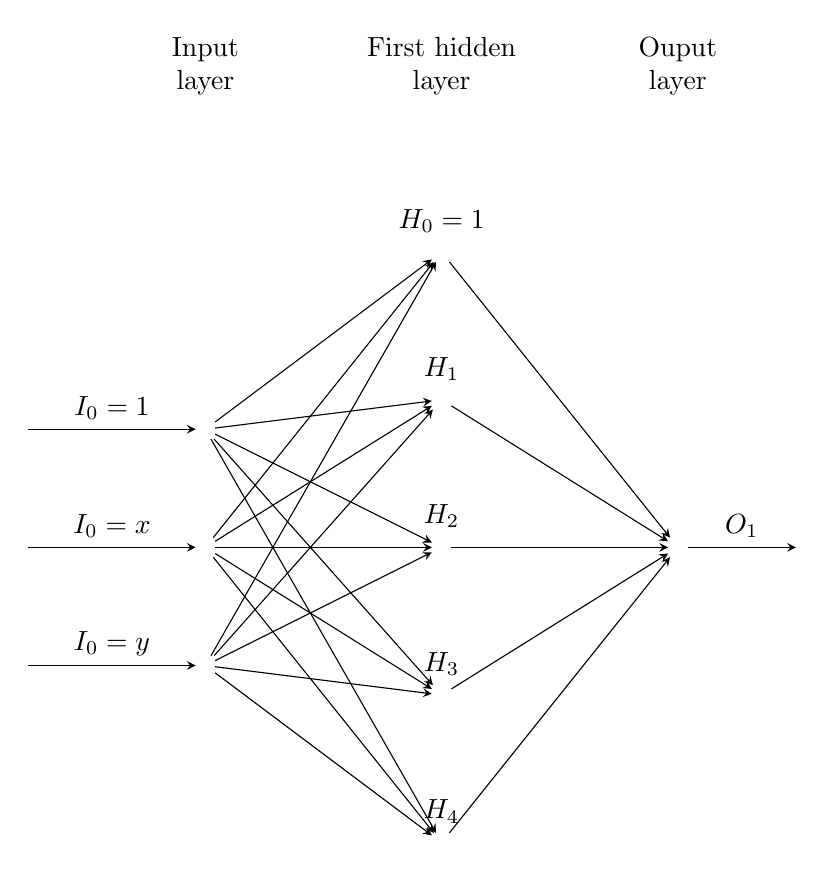
\begin{tikzpicture}[x=1.5cm, y=1.5cm, >=stealth]

\foreach \m/\l [count=\y] in {0,1,2}
  \node [every neuron/.try, neuron \m/.try] (input-\m) at (0,0.25-\y) {};

\foreach \m [count=\y] in {0,1,2,3,4}
  \node [every neuron/.try, neuron \m/.try ] (hidden-\m) at (2,2-\y*1.25) {};

\foreach \m [count=\y] in {1}
  \node [every neuron/.try, neuron \m/.try ] (output-\m) at (4,-0.75-\y) {};

\draw [<-] (input-0) -- ++(-1.5,0) node [above, midway] {$I_0=1$};
\draw [<-] (input-1) -- ++(-1.5,0) node [above, midway] {$I_0=x$};
\draw [<-] (input-2) -- ++(-1.5,0) node [above, midway] {$I_0=y$};

\node [above] at (hidden-0.north) {$H_0 = 1$};

\foreach \l [count=\i] in {1,2,3,4}
  \node [above] at (hidden-\l.north) {$H_\l$};

\foreach \l [count=\i] in {1}
  \draw [->] (output-\i) -- ++(1,0)
    node [above, midway] {$O_\l$};

\foreach \i in {0,...,2}
  \foreach \j in {0,...,4}
    \draw [->] (input-\i) -- (hidden-\j);

\foreach \i in {0,...,4}
  \foreach \j in {1}
    \draw [->] (hidden-\i) -- (output-\j);

\foreach \l [count=\x from 0] in {Input, First hidden, Ouput}
  \node [align=center, above] at (\x*2,2) {\l \\ layer};

\end{tikzpicture}

\caption{\textbf{Polygon A classification - neural network layout}}
\end{figure}

\subsection*{Weights}
\begin{enumerate}
\item The coordinates of the point we are classifying are in the form: $(x,y)$. Therefore, we need to put them in the input layer along with a one: $I_0=1, I_1=x, I_2 = y$.
\item As for the first hidden layer, we need a neuron for each edge of the polygon. Starting from the upper-left edge (as seen on Figure \ref{polygons}) and going along the polygon in counter-clockwise order, each neuron decides if the input point is below/above the line that passes through the corresponding edge.
\begin{enumerate}
\item \underline{$H_1$}: \textbf{1} if below the line that passes through the first edge; otherwise
\textbf{0}
\item \underline{$H_2$}: \textbf{1} if above the line that passes through the second edge; otherwise \textbf{0}
\item \underline{$H_3$}: \textbf{1} if above the line that passes through the third edge; otherwise \textbf{0}
\item \underline{$H_4$}: \textbf{1} if below the line that passes through the fourth edge; otherwise \textbf{0}
\end{enumerate}
For example, for $H_1$ we need to make sure that the value of the neuron corresponds to the fact that the following inequality holds (approximately): $y < 1.116 * x + 1.170$ as $y = 1.115 * x + 1.170$ is the equation of the line that passes through the upper-left edge. Now, we can transform this inequality into vector form and normalise it by dividing by the biggest absolute value ($1.170$ in this case): 
\begin{align}
     \begin{bmatrix}
           1 \\
           x \\
           y
         \end{bmatrix} \bullet \begin{bmatrix}
           1.170 \\
           1.116 \\
           -1
         \end{bmatrix} &> 0 \Leftrightarrow \begin{bmatrix}
           1 \\
           x \\
           y
         \end{bmatrix}  \bullet \begin{bmatrix}
           1 \\
           0.954 \\
           -0.855
         \end{bmatrix} > 0
  \end{align}
Now, we can take the vector on the right as the weight vector for $H_1$. Once the step function is applied, this will ensure that the requirements for the output of $H_1$ set above are met.
For $H_2, H_3, H_4$, we can proceed in an equivalent fashion.
  
\item Finally, the output layer weight are constructed so that the output is $1$ if and only if $H_1 = H_2 = H_3 = H_4 = 1$. This can be achieved by taking $[-\frac{4}{5}, \frac{1}{4}, \frac{1}{4}, \frac{1}{4},\frac{1}{4}]$ as the weight vector. If at least one of $H_1, H_2, H_3, H_4$ is equal to $0$, then the following will hold (as the rest can only sum up to $\frac{3}{4}$ at maximum, which is smaller than $\frac{4}{5}$):
\begin{align}
     \begin{bmatrix}
           1 \\
           H_1 \\
           H_2 \\
           H_3 \\
           H_4 
         \end{bmatrix} \bullet \begin{bmatrix}
           -4/5 \\
           1/4\\
           1/4\\
           1/4\\
           1/4
         \end{bmatrix} & < 0
\end{align}
\end{enumerate}

\begin{figure}[!htb]
\centering
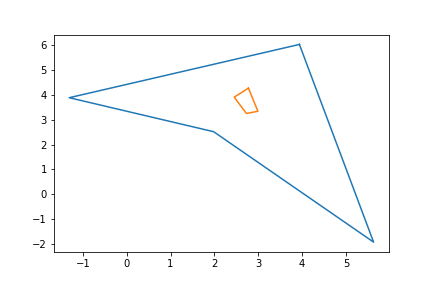
\includegraphics[scale=0.8]{task2_polygons.png}
\caption{\textbf{Polygons A, B}; The A polygon is in orange, the B polygon is in blue.}
\label{polygons}
\end{figure}

\newpage

\subsection*{2.10 - Different decision regions for sigmoidal/step functions}


\end{document}

